\documentclass{scrartcl}

\usepackage[utf8x]{inputenc}
\usepackage{array}
\usepackage{tabularx}
\usepackage{multirow}
\usepackage{graphicx}
\usepackage{booktabs}
\usepackage{caption}
\usepackage{subcaption}
\usepackage{titling}
\usepackage{xcolor}
\usepackage{amsmath}
\usepackage{amsfonts}
\usepackage{multicol}
\usepackage{wrapfig}

\usepackage[a4paper, margin=.9in]{geometry}
\usepackage{tikz}
\usetikzlibrary{shapes,decorations,arrows,calc,arrows.meta,fit,positioning}
\tikzset{
    -Latex,auto,node distance =1 cm and 1 cm,semithick,
    state/.style ={ellipse, draw, minimum width = 0.7 cm},
    point/.style = {circle, draw, inner sep=0.04cm,fill,node contents={}},
    bidirected/.style={Latex-Latex,dashed},
    el/.style = {inner sep=2pt, align=left, sloped}
}

\setlength{\droptitle}{-7.5em}

\title{Causal Inference for Policy Evaluation\\
\Large{Assignment 4}}
\author{Marco Gortan, Felix Schulz, Benjamin Weggelaar}
\date{\today}

\newcommand{\marco}[1]{\textcolor{red}{#1}}
\newcommand{\felix}[1]{\textcolor{cyan}{#1}}
\newcommand{\benji}[1]{\textcolor{green}{#1}}

\begin{document}

\maketitle



\subsection*{Question 1}

\paragraph*{(a)}
% Estimate the treatment effects using the RD method for municipalities above or below the median value of income. Use a linear control for the running variable and options kernel=“triangular” and bwselect=“mserd”. Do not include any covariate. Report the point estimates and s.e. for each sub-sample and explain what the options kernel=“triangular” and bwselect=“mserd” do.
With the option \texttt{kernel="triangular"} the weights of the observations decrease linearly with distance from cutoff to trade-off between power (more observation) and bias. The option \texttt{bwselect="mserd"} chooses the bandwidth that minimizes the mean squared error for estimating the treatment effect at the cutoff.

\paragraph*{(b)}
% Repeat the estimation in point (a), but now control for all the covariates in COVS.Report the point estimates and s.e. for each sub-sample. Compare the results form point (a) and (b) and comment. Should we expect them to be similar?
If the groups above/below the thresholds have similar characteristics, we should expect no differences when adding covariates. This is the case for the sub-sample below median income (Table \ref{tab:Ex1ab}). However, the estimates and their significance are different for the above median sub-sample, suggesting that we have discontinuity in covariates that affect the outcome.

\begin{table}

\caption{\label{tab:tab:rdd_results}RDD Estimates for Below and Above Median Income}
\centering
\begin{tabular}[t]{ccccccc}
\toprule
\multicolumn{1}{c}{ } & \multicolumn{2}{c}{Below Median} & \multicolumn{2}{c}{Above Median} & \multicolumn{2}{c}{RDD Test} \\
\cmidrule(l{3pt}r{3pt}){2-3} \cmidrule(l{3pt}r{3pt}){4-5} \cmidrule(l{3pt}r{3pt}){6-7}
 & Estimate & SE & Estimate & SE & Estimate & SE\\
\midrule
Without covariates & 0.50 & 2.01 & 1.01 & 4.05 & -610.97 & 52.47\\
With covariates & -0.14 & 1.59 & 5.61 & 1.90 & NA & NA\\
\bottomrule
\end{tabular}
\label{tab:Ex1ab}
\end{table}



\paragraph*{(c)}
% Meyersson argues that the treatment effect could be larger in poorer municipalities. Provide some intuition as to why this might be the case. Are the RD estimates from points (a) and (b) in line with this reasoning?
Poorer areas are more likely to be more religiously conservative. There, Islamist municipalities would not enforce secular barriers to school entry like the headscarf ban, increasing schooling for girls. RD estimates \underline{do not} support this reasoning; actually, the specification with covariates above median income supports the opposite.   

\paragraph*{(d)}
%What would happen to your estimator if you halved the bandwidth around the cutoff?
Halving the bandwidth around the cutoff implies that we have less observations (so less power, more variance in the estimate) but we reduce the bias that might be induce by other factors, as very close to the margin municipalities might be more similar to each other.  


\paragraph*{(e)}
%  Conduct a suitable check that there is no selection in terms of household income at the cutoff. Comment on the result, the validity of an RD approach, and what we can learn from the estimates in points (a) and (b)
The group "RDD Test`` in Table \ref{tab:Ex1ab} shows the estimate of an RD regression where the dependent variable is the income of the municipality and the running variable is the winning margin. The result tells us that we have income discontinuity at the cutoff, since municipalites where the Islamic party wins by a small margin are much poorer compared to those where the Islamic party loses by a small margin, pointing to a possible electoral result manipulation in poor municipalities to favor the Islamic party. This violates the RD continuity assumption and suggests potential bias. The estimated treatment effects in (a) and (b) could partly reflect pre-existing income differences rather than the Islamic party’s victory per se.

\subsection*{Question 2} % Validity checks

\paragraph*{(a)}
%  Perform the McCrary (2008) density discontinuity test for the running variable and plot the frequency of the running variable. Describe the results and explain whether they are indicative for bunching behavior
Figure \ref{fig:threshDens} shows clear evidence of bunching behaviour. \input{output/other/4_mccrary_test.txt}It is indeed twice more likely to find municipalities with an electoral margin slightly above than the cutoff compared to slightly lower the cutoff, suggesting possible manipulation of the running variable. In an appropriate RD design, we should instead observe a continuous line. 

\paragraph*{(b)}
%  Check whether municipalities differ in terms of the percentage of population above 60 (ageshr60) and below 19 (ageshr19) by running separate RD estimations. As in question 2, use a linear control for the running variable and options kernel=“triangular” and bwselect=“mserd”. Report the point estimates and standard errors along with the corresponding p-values. What conclusions do you draw with regard to sorting in covariates? Briefly comment
Results are displayed in Table \ref{tab:Ex2b}. The estimate for the RDD for \textit{Age share below 19} suggest the young municipalities, i.e. those with a higher share of people with age below 19, are those that are more likely to manipulated results. The estimate of 6.7 is indeed almost statistically significant at the 5\% level.   

\begin{figure}
  \begin{minipage}[b]{.45\linewidth}
    \centering
    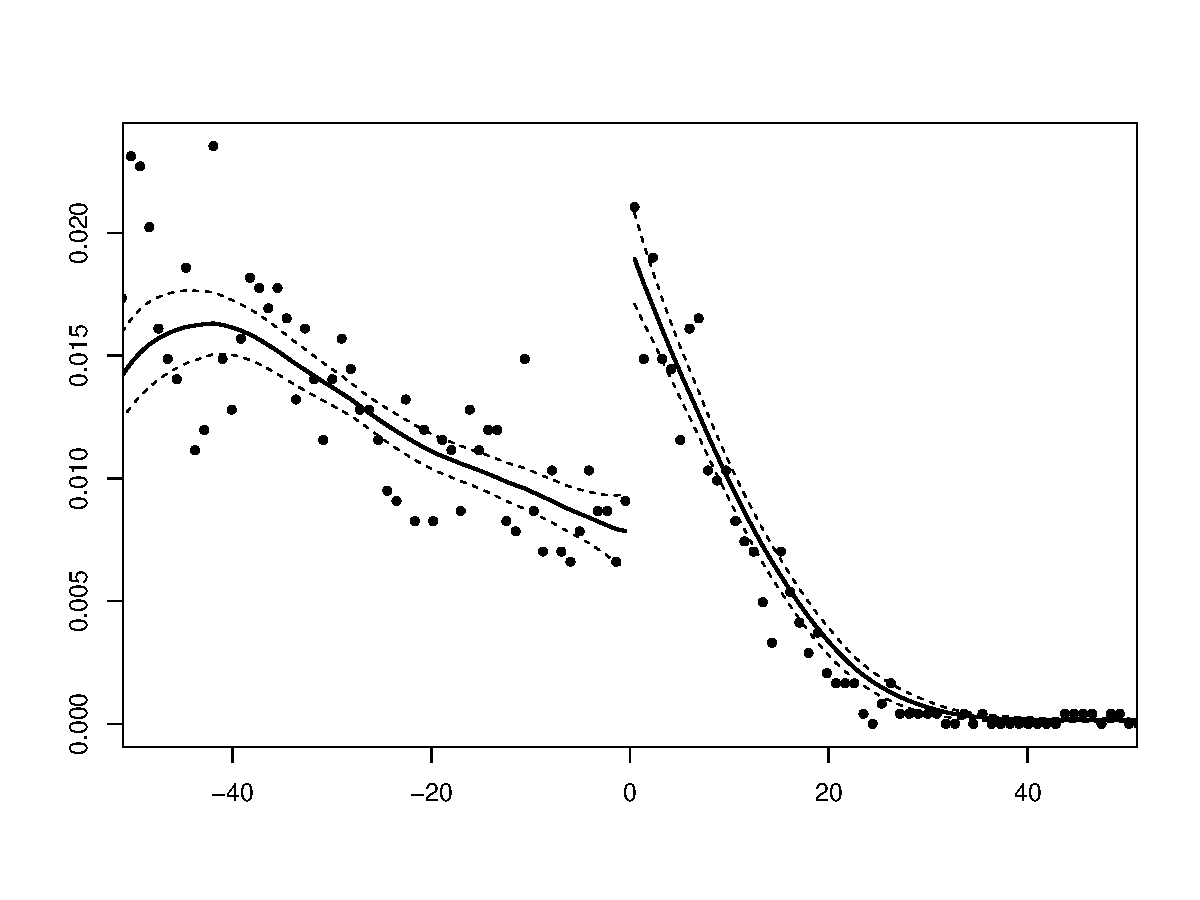
\includegraphics[width=\linewidth]{output/figures/4_density_test.pdf}
    \captionof{figure}{Density of the running variable}
    \label{fig:threshDens}
  \end{minipage}\hfill
  \begin{minipage}[b]{.45\linewidth}
    \centering
    \captionof{table}{RDD estimates for age demographics}
    \label{tab:Ex2b}
    \vspace{.5em}                   % small gap between caption and tabular
    \begin{tabular}{lccc}
      \toprule
      Variable            & Estimate & SE    & $p$-value\\
      \midrule
      Age share $\ge 60$  & –1.620   & 1.508 & 0.283\\
      Age share $\le 19$  &  6.722   & 3.480 & 0.053\\
      \bottomrule
    \end{tabular}
  \end{minipage}
\end{figure}

\paragraph*{(c)}
%  Given the results from (1d), (2a) and (2b), can we use an RD approach to estimate the desired treatment effect? Briefly make the case for or against the RD design by discussing the validity of each of the identifying assumptions.
We observe that small victory margins happen in (i) poor municipalities and (ii) municipalities with a higher share of young people. Discontinuities in wealth or age imply that municipalities barely won by the Islamic party differ \emph{ex ante} from barely losing ones. In other words, treatment is no longer “as good as randomly assigned” in a neighborhood of the cutoff. If the manipulation is solely along observables, including controls might alleviate these concerns. Given that this is highly unlikely, the observation of this bunching behavior leads us to conclude that a naïve RDD application is invalid. 

\subsection*{Question 3} % Simulation


\paragraph*{(b)}
%  Since we generate the data ourselves, we know the value of the treatment effect that we will then try to recover. What is the value of the treatment effect that we are interested in?
Since $D^{sim}$ is the variable that indicates being above the cutoff, we expect the treatment effect to be $-5$.
 
\paragraph*{(c)}
%  Present a table with the RD point estimates, the RD s.e., the RD bandwidth, the OLS estimates and the OLS robust s.e. for a sample size of 5,000, 10,000 and 20,000. What do the results suggest about the precision of the RD estimator compared to OLS? Explain why this is the case
The precision of the OLS estimator is always better compared to the precision of the RD estimator. This is due to the fact that (i) OLS is using the entire sample and while RD is not and (ii) the RD bandwidth also shrinks as the sample increases. Therefore, the OLS estimator converges faster to the true value. 


\begin{table}

\caption{\label{tab:tab:sim_results}Simulation Results for Different Sample Sizes}
\centering
\begin{tabular}[t]{cccccccccc}
\toprule
\multicolumn{1}{c}{ } & \multicolumn{3}{c}{RD} & \multicolumn{6}{c}{OLS} \\
\cmidrule(l{3pt}r{3pt}){2-4} \cmidrule(l{3pt}r{3pt}){5-10}
Sample & Estimate & SE & BW & D Estimate & D SE & X Estimate & X SE & DX Estimate & DX SE\\
\midrule
5000 & -4.83 & 0.71 & 16.33 & -4.66 & 0.40 & 0.51 & 0.01 & -1.02 & 0.01\\
10000 & -5.43 & 0.59 & 14.50 & -5.08 & 0.29 & 0.51 & 0.01 & -1.02 & 0.01\\
20000 & -5.43 & 0.42 & 14.10 & -5.31 & 0.20 & 0.50 & 0.00 & -0.99 & 0.01\\
\bottomrule
\end{tabular}
\end{table}




\paragraph*{(d)}
%   Given the data generating process in point (a), is the OLS estimator biased or unbiased for the treatment effect of interest? Why? Would you use the RD or the OLS estimates from point (c) for inference?
Given the data generating process, the OLS estimator in an unbiased estimator of the treatment effect of interest since we are estimating a model that we know is at the base of the data generating process. \\

For inference, when we are interested in predicting values that might fall outside the bandwidth, it is better to use OLS, which fits the parameters using all the observations.


\subsection*{Question 4} % PhD only 

\paragraph*{(a)}
%   How would you define the running variable based on this data and how would this coarser measurement affect its quality? Could you still estimate a valid RDD effect? Explain why or why not

We can construct the running variable the same way as before. Namely, the win/loss margin is the vote share of the Islamic party minus the vote share of the secular party. The coarser measurement reduces precision and turns a continuous running variable into a discrete one with gaps (e.g., -4\%, -2\%, 0\%, +2\%, etc.). We are still able to retrieve a sharp RDD, because for margins that are rounded to 0\%, we can complement our data with information on the winner of the election (since this information is public). Therefore, even for margins at 0\%, we can still allocate the winners (Islamic parties) to the right part of the cutoff and losers to the left part. This could be achieved by creating a dummy variable. Nevertheless, we believe this reduces the precision of the estimate, and causes bias. The rounding causes measurement error that increases the standard error. Furthermore, we believe it causes a biased estimate due to endogeneity. Suppose that instead of observing the true variable \( x_i^* \), what is actually observed is 

\[
x_i = x_i^* + \nu_i
\]

where \( \nu_i \) is the measurement error caused by the rounding. In this case, a model given by

\[
y_i = \alpha + \beta x_i^* + \varepsilon_i
\]

can be written in terms of observables and error terms as:
\begin{align*}
y_i &= \alpha + \beta (x_i - \nu_i) + \varepsilon_i 
 =  \alpha + \beta x_i + (\varepsilon_i - \beta \nu_i) \\
    &= \alpha + \beta x_i + u_i \quad \text{(where } u_i = \varepsilon_i - \beta \nu_i \text{)}
\end{align*}

Since both \( x_i \) and \( u_i \) depend on \( \nu_i \), they are correlated. This violates the OLS assumption that the regressors are uncorrelated with the error term. As a result, the estimation of \( \beta \) will be biased.


\paragraph*{(b)}
%   Would your conclusion change if you did not need to construct the running variable yourself but got it delivered as a rounded variable by the statistical office (still in increments of 2 percentage points)? Would the quality of your estimates be affected by the coarser measurement and if yes, how?

In question 4a) we receive the rounded electoral votes shares, and can construct the running variable by taking the difference. In this new scenario, we are not sure whether the margins were first rounded and then the difference was taken (option 1), or the other way around (option 2). In order to explore if this would change the measurement error in anyway, we slightly change the simulation exercise in 3, in order to simulate the two voter shares separately. Figure 2 shows how the measurement error differs between the two ways of constructing the running variable: 


\begin{figure}[htbp]
    \centering
    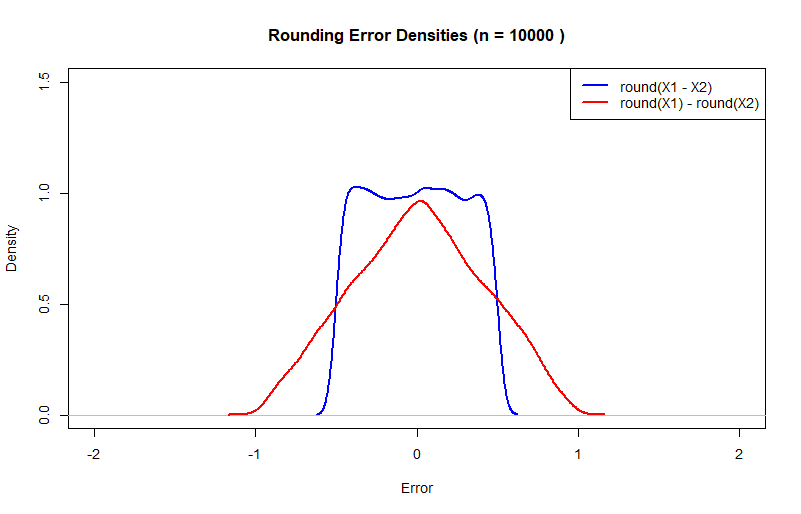
\includegraphics[width=0.4\textwidth]{output/figures/rounding_error.png}
    \caption{Differences in simulated measurement errors}
    \label{fig:your_label}
\end{figure}

Although the shape is different, the expected values of the errors would be the same and we still have $Cov(x_i,u_i) \neq 0$, causing endogeneity. Therefore, we believe the quality of the estimate to remain the same. 




\end{document}